\documentclass[12pt]{book}
\usepackage[nottoc,notlot,notlof]{tocbibind}
\usepackage[spanish,mexico]{babel}	
\usepackage[utf8]{inputenc} %latin1
\usepackage[T1]{fontenc}
\usepackage{pslatex}
\usepackage{graphicx}
\usepackage{setspace}
\usepackage{xcolor}
\definecolor{azul}{rgb}{0.36, 0.54, 0.66}
\usepackage[left=2.5cm, top=3.5cm, bottom=2.5cm, right=3cm]{geometry}


\begin{document}

	    \begin{titlepage}
    	\begin{center}
    		{\huge \textbf{Universidad de Colima}}\\
    		\vspace{1mm}
    		{\Large \textbf{Educación con responsabilidad social}}
    		\vspace{1mm}
    		\begin{figure}[h]
    			\centering
    			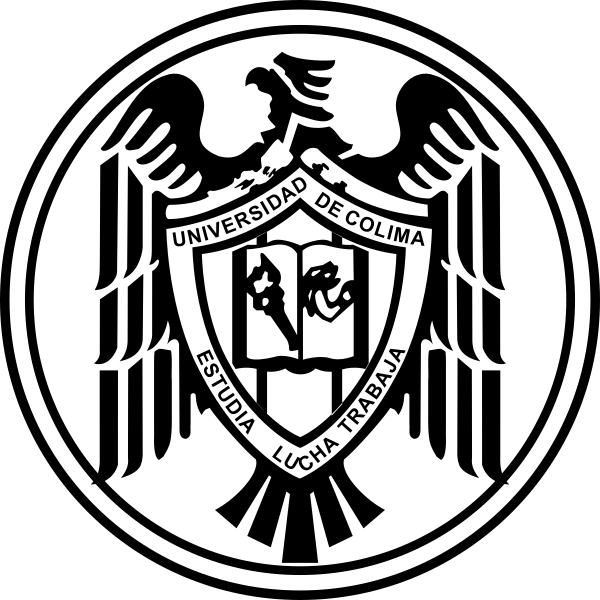
\includegraphics[height=5cm]{./src/logoUcol.png}
    		\end{figure}
    		
    		{\LARGE \textbf{Facultad de Ingeniería Electromecánica}}\\ 
    		
    		\vspace{5mm}
 
    		\begin{spacing}{1}
    			{\LARGE \textsc{Entrenador de Exámenes (Aplicación Web y Móvil de Evaluación y Entrenamiento Educacional)} }
    		\end{spacing}
    		
    		\vspace{5mm}
    		
    		{\LARGE \textbf{TESIS}}\\
    		\vspace{2mm}
    		{\large \textsc{Para obtener el titulo de:}}\\
    		\vspace{3mm}
    		{\LARGE \textbf{INGENIERO DE SOFTWARE}}\\
    		\vspace{1cm}
    		{\Large \textsc{Presentan}}\\
    		\vspace{5mm}
    		{\large \textbf{EDGAR JAVIER OROZCO MONRROY}}\\
    	
    		{\large \textbf{ROBERTO DAMIAN LEÓN HERNANDEZ}}\\
    		\vspace{1cm}
    		{\Large \textsc{Asesores:}}\\
    		\vspace{5mm}
    		{\large \textbf{JUAN PABLO MARTÍNEZ VARGAS}}\\
    		{\large \textbf{ENRIQUE CARLOS ROSALES BUSQUETS}}\\
    		\vspace{3.5mm}
    		\vfill
    		{\Large \textbf{Manzanillo, Colima\\ Octubre 2022}}
    		
    	\end{center}
    \end{titlepage}

	\frontmatter
	\chapter*{Agradecimientos}
 	\chapter*{Abstract}
      
	\chapter*{Resumen}
         
	\tableofcontents
	\listoffigures
	\listoftables
	\mainmatter
	\chapter{Introducción}
	{\normalsize Actualmente la tecnología en las aulas esta más presente que nunca, el uso de dispositivos móviles entre alumnos se volvió más una necesidad que un lujo, en muchas universidades se implementan trabajos que funcionan de forma online, lo que cuenta con muchas ventajas frente a métodos tradicionales, por ello en los últimos años a causa de la pandemia ocasionada por el COVID-19 la mayoría de la población estudiantil tuvo que aprender de forma forzada como trabajar haciendo uso de sistemas en línea, a partir de esto surgieron aplicaciones web y móviles que tienen el objetivo de mejorar el desempeño de las clases que imparte el maestro hacia el alumno en un medio asíncrono. La mayoría de las aplicaciones eficientes orientadas a la educación cuentan con un sistema multiplataforma, en su mayoría orientados a un sistema web y móvil, esto permite que el maestro se pueda desempeñar de una mejor manera, ya que el uso de una computadora de escritorio puede representar mayor comodidad que un dispositivo móvil, generalmente por el tamaño de la pantalla, se representa una mayor visualización de la información en una computadora de escritorio que en un dispositivo móvil, en cambio la mayoría de los alumnos cuentan con un dispositivo móvil con conexión a internet, cabe mencionar que cuando se trata de evaluar al alumno, este ultimo solo requiere de un dispositivo móvil ya que el cuestionario se suele encontrar en un sitio web o una aplicación. En esta tesis presentamos una propuesta para apoyar a universitarios que quieran mejorar su desempeño al momento de realizar el examen de egreso EGEL. Para realizar esta aplicación se busco una biblioteca que nos permitiera desarrollar para la plataforma web, iOS y Android, el candidato perfecto es React JS, este se encuentra disponible para desarrollar en varias plataformas, también cabe mencionar que cuenta con buen soporte y una gran comunidad, lo que nos da una referencia sobre productos finales. La necesidad de una plataforma en formato web surge mayormente por el requerimiento de funcionalidades dirigidas al profesor, estas son como la elaboración de cuestionarios, la redacción de información y la aplicación de tareas a pesar de que también se encuentran disponibles estas últimas en la versión móvil, se tiene en cuenta que el maestro trabaja de mejor forma en un sitio web, por el hecho de que este se puede ejecutar en cualquier ordenador usando una sesión propia. La necesidad de la plataforma móvil esta dirigida hacia el alumno, las funcionalidades principales de este están dirigidas a la versión móvil, esta decisión es tomada teniendo en cuenta que la mayoría de los alumnos tienen un dispositivo Android o iOS, en este es posible responder formularios, entregar trabajos y leer información redactada por el maestro, incluso el alumno no necesita tener conexión a internet obligatoriamente ya que la información publicada por el tutor es almacenada en la aplicación móvil.}
	\subsection{Trasfondo del proyecto}
	{\normalsize Este proyecto fue retomar un proyecto de tesis que los ingenieros de software de una generación posterior intentaron desarrollar pero fue dejado a la deriva, intentando así retomar la problemática original, adaptándola a nuestra visión del proyecto además de agregar funcionalidades que creemos pueden generar un producto bastante completo y que satisface las necesidades y requerimientos esperados pues en realidad el examen de egreso es algo que no muchos alumnos a lo largo de todas las carreras pasan con facilidad, crear una plataforma de estudio y retroalimentación sobre el EGEL es algo muy útil y requerido en estos tiempos.
		\\
	Es importante comentar que el desarrollo móvil es casi un proyecto personal que se viene trabajando inclusive meses antes de la elección por esta tesis, por ello nos resulto desafiante el querer realizar el entorno multiplataforma lo cual esperamos desarrolle nuestras habilidades como ingenieros, en un principio este fue elaborado con React Native, tecnología enfocada únicamente móvil, pero fue migrado para React web el cual tiene la capacidad de ser compilado de manera nativa también en móvil con ciertas herramientas. }
	\subsection{Problema}
	{\normalsize En los últimos el examen EGEL ha funcionado como requerimiento principal para medio de graduación en los alumnos de licenciatura actualmente se presentan deficientes medios de estudio para este examen y es necesario actualizarlos,  el problema general es realizar una aplicación que apoye a los próximos universitarios estudiantes de licenciatura a realizar prácticas sobre la aplicación del examen EGEL. Esta problemática se desborda en lo que es estudiante puede y no realizar en un entorno de comunicación y prácticas en línea por lo cual se decide abordar mas de este problema programando prácticamente una guía gratuita y de libre acceso que cualquier universitario podría consultar. \\ 
    Aún existen muchos estudiantes que no disponen de una computadora, en cambio sí cuentan con una red de acceso a internet y pierden ese nivel de efectividad dentro de las páginas que son más novedosas si entramos desde una computadora. La gran mayoría de estudiantes cuentan con un dispositivo móvil propio esto nos da una gran oportunidad para abarcar ese espacio vacío para practicar próximas evaluaciones profesor-alumno y evaluar de manera dinámica.
    \\
    Sabemos que el Examen General para el Egreso de la Licenciatura es un pilar importante para la graduación de todo aquel estudiante que desee recibirse, existen actualmente guías para prácticamente cualquier carrera pero o estas cuestan mucho dinero o simplemente son reactivos variados sobre temas específicos además de no retro-alimentar en tiempo real a el alumno sobre sus conocimientos. Necesitamos encontrar una manera de otorgar a los alumnos una aplicación amigable además de fácil acceso por que así mejorarían las posibilidades de que las próximas generaciones de licenciados tengan con mayor facilidad su pase a ser acreedores del titulo por el cual trabajaron años. 
	}
	
	\subsection{Objetivo}
	{\normalsize El objetivo para el desarrollo de este proyecto es generar una aplicación web multiplataforma que ayude estudiantes de todo nivel académico de manera gratuita y accesible a prepararse para el examen EGEL pues actualmente las estrategias de estudio que se tienen son deficientes y cuestan dinero. }
 
	\subsubsection{Objetivos específicos}
	{\normalsize \begin{itemize}
			\item Creación de una interfaz, atractiva, amigable y con funciones que apoyen a el alumno así como fomentar su aprendizaje con práctica por medio de mostrarle sus puntos mas débiles con una ponderación. 
			\item Conexión entre funciones de aplicaciones móviles/web las cuales se complementen. El alumno puede estar en el móvil, así como el profesor en web y viceversa menté, creando así una aplicación completa que sea un todo. 
			\item Programar en un entorno enfocado en Front-End, lo cual beneficia la accesibilidad con la que cuenta la aplicación y a su vez lo convierte en un producto de muy fácil entendimiento. 
			\item Usar los conocimientos de Javascript para poder emplear el framework de React lo cual nos permitirá la aplicación multiplataforma y el uso asíncrono.
     \end{itemize}}

        \subsubsection{Objetivos de investigación} 
        {\normalsize \begin{itemize}
            \item Aprender el funcionamiento y emplear el framework React. 
            \item Enfocarse en adaptar un estilo de producción en un Framework web con un conjunto de marcos tecnológicos como lo son Firestorage del lado de almacenamiento de datos por medio de una base de datos no SQL y Node.js que permite la ejecución de JavaScript del lado del servidor y no estrictamente en el navegador. 
            \item Recopilar diferentes bancos de preguntas y reactivos además de guías EGEL de múltiples carreras nivel licenciatura para tener la capacidad de realizar exámenes de diferentes áreas. 
            \item Investigar la estructura de preguntas presentes en las pruebas EGEL.
            \item Encontrar la metodología que mejor se adapte a nuestro estilo de trabajo y necesidades. 
            \item Indagar en métodos de retroalimentación que motiven a los usuarios a seguir con su aprendizaje. 
        \end{itemize}}
        
	\subsection{Justificación}
	{\normalsize 	Los motivos los cuales hicieron posible el desarrollo de este proyecto son las pocas o casi nulas aplicaciones que existen para poder practicar de manera abierta y gratuita la prueba EGEL para obtener el titulo en cualquier carrera universitaria. Existen cada día mas Universidades y acceso a la educación lo cual incrementa el numero de estudiantes que presentaran esta prueba contando actualmente solo con guías de paga las cuales no proporcionan retroalimentación y no son intuitivas ademas de carecer de la capacidad de ser contestadas en cualquier momento y forma.}
	
\subsection{Metodología }
	{\normalsize En el presente proyecto el objetivo fue realizar en el menor tiempo posible todos las secciones planeadas del software, se usa la metodología ágil, la cual consta en  el análisis del problema , posteriormente se planea emplear el diseño:}
	\begin{itemize}
		\item Diseño back-end llevado acabo con NodeJS que cuenta con una alta compatibilidad con el front-end usando al mismo lenguaje Javascript siendo este entorno muy escalable equipado ya con características para el manejo de cuentas y consultas. NodeJS es muy veloz gran cantidad de compatibilidad con APIs ademas de el soporte multiplataforma que necesitamos pues tiene que ser móvil/web. 
		
		\item El diseño de base de datos sera llevado acabo con Firebase optando por dejar de lado MySQL pues el primero resulta de mas fácil el manejo multiplataforma ademas de que el manejo de datos no resulta tan complejo u abstracto como para emplear relaciones. Firebase cuenta con el uso de documentos del tipo JSON, lo cual beneficia a la hora de estructurar objetos como los exámenes pudiendo así compartir plantillas y estandarizar el crear, usar y contestar exámenes para que estos sean lo mismo para cada usuario sea el uso que se desee. 
		
		\item Para el diseño del front-end se busco que el producto cuente con una alta accesibilidad, dejando así de lado los diseños propios y optando por basarse en un estándar como lo es el diseño dashborad de muchas aplicaciones web con una navegación intuitiva, es ciertamente que el tratado de la accesibilidad mejora muchísimo como una aplicación es conservada si esta es tratada adecuadamente desde el principio. 
		
		La metodología empleada continua con el apartado del desarrollo el cual se llevo acabo a lo largo de los meses posteriores contando así con el trabajo móvil y web lo cual resulto en arduas semanas de trabajo e investigación pues este modelo de trabajo sugiere realizar un "Research-Development" (investigación-desarrollo) a la par lo cual incrementa la velocidad a la cual es posible programar y desarrollar las estructuras de backend y frontend presentes en el proyecto. \\
		La metodología ágil concluye con el testing e implementación, lo cual completa un circulo que se intenta repetir ante cada avance en el proyecto subdividiendo a este en módulos a desarrollar por ello el trabajo de desarrollo nunca termina y se intenta llegar a la mejor versión de este.
	\end{itemize}

        \subsubsection{Módulos de la metodología planeados (Ágil)}
        {\normalsize \begin{itemize}
            \item \textbf{Modelado y planificación:} Aquí es cuando mas se trabaja en el área teórica, de investigación y modelado desde la estructura de datos como en el diseño de la base de datos, es cuando realmente es importante entender como funcionan los datos pues a partir de aquí es cuando se comenzaran a manipular para darle forma a la aplicación.
            
            \item \textbf{Backlog:} El cual sera la lista de prioridades por programar con su respectiva importancia e impacto en el proyecto. Así el desarrollo estará mejor organizado.

            \item \textbf{Sprint:} Sera el momento en el que el equipo completo de trabajo se pondrá trabajar de lleno en el desarrollo siguiendo lo planeado en el modelado y backlog previamente planificados.
            Es cuando realmente se comenzaran a ver reflejados commits en el repositorio y avanzara lo tangible del software. Aquí veremos reflejadas (Pantallas, conexión con base de datos, lanzamiento en un servidor y diferentes módulos de la aplicación trabajados)

            \item \textbf{Iteración:} Es el momento donde se hará un análisis a lo realizado dándole puntos débiles, posibles mejoras y se trabajara en poner en marcha todo lo mejorable desde el modelado dando de nuevo vida al desarrollo para poner en marcha el próximo sprint. 

            \item \textbf{Lanzamiento:} Es la etapa donde se tiene por concluido el proyecto, es cuando todos los participantes de esta investigación instrumental quedamos conformes para ser presentado. 

        \end{itemize}}


 
	\chapter{Marco Teórico}
	\section{Estado del arte}
        {\normalsize En este apartado se describen los principales documentos que son mas relacionados al proyecto que se llevo acabo, estos ademas de fungir como parte aguas del proyecto son parte de inspiración pues prácticamente continuamos o actualizamos funciones que otras personas han desarrollado en artículos o tesis, es mejorar y hacer nuestro algo que tiene en desarrollo mucho tiempo. }
	\begin{enumerate}
		
		\item \textbf{Sistema de evaluaciones
		en línea como herramienta para los niveles de
		educación media superior}.\\
		{\normalsize Según los autores la problemática principal a la que se afrontaron fue el generar una solución a la cuestión del por que los profesores obtienen siempre los mismos resultados promedio al evaluar a los estudiantes mediante prácticas tradicionales, cuestionables si realmente las herramientas con las que cuentan los docentes son realmente eficaces a la hora de presentar sus evaluaciones, en el articulo \cite{brambila2015sistema} se menciona \textit{"Hoy  en día el  uso  de  las  tecnologías en  línea  en  las  instituciones  educativas  se han convertido en una herramienta de gran importancia por la facilidad y rapidez con la que se realizan  todas  las  operaciones  de  cualquier índole."}}	
         
         {\normalsize La próxima tesis por realizar está enfocada en mejorar el funcionamiento de esta aplicación y nuevas funciones añadidas para crear un producto más capaz y actual, principalmente enfocado en herramientas como entregar tareas y entrenar para exámenes.}
	
	    \item \textbf{El modelo flipped classroom \\}
	    {\normalsize El articulo menciona y aborda sobre la problemática a la manera que el tipo de aprendizaje generara alumnos mas atentos, profesionales mejor preparados y aumentara el nivel educativo inclusive a nivel país. \cite{aguilera2017modelo} en su articulo aporta al aprendizaje de manera en linea : " \textit{El aula invertida o flipped classroom es un método de enseñanza cuyo principal objetivo es que el alumno/a asuma un rol mucho más activo en su proceso de aprendizaje que el que venía ocupando tradicionalmente." }} 
	    
	    {\normalsize Me parece buena propuesta, creo que así debería ser la manera de educar, obviamente conservando la enseñanza tradicional, pero innovando más y ciertamente sacando el mayor provecho a las tecnologías de la información. Se buscará adaptar este modelo de educación enfocándolo hacia el proyecto de aplicación alumno-maestro que estamos desarrollando.}
	    
	    \item \textbf{Tecnologías y nuevas tendencias en educación: aprender jugando. El caso de Kahoot \\}
	    {\normalsize Describe el como el juego ha hecho que la
	    	educación mejore, mediante el uso de estrategia de
	    	competencia, y se compara estos resultados mediante la
	    	educación tradicional. Posiblemente el uso de juegos es la mejor manera
	    	de educación posible, se ha demostrado que usualmente las
	    	personas que juegan videojuegos en específico por ejemplo
	    	de estrategia alcanzan un nivel de concentración
	    	y lucidez difícilmente presentada en modelos de educación
	    	tradicionales. \cite{navarro2017tecnologias} en el articulo referente a las nuevas tecnologías y las estrategias de aprendizaje se menciona : " \textit{ Los  modelos  de enseñanza  tradicionales  dan  paso a  nuevas  formas  de  aprendizaje que tienen   como   telón   de   fondo   las   nuevas   tecnologías   que   están cambiando tanto el proceso de aprendizaje como el rol de estudiantes y docentes." }} 
	    
	    {\normalsize Me parece buena propuesta, los videojuegos como
	    	Kahoot que permiten la evaluación general aventajando
	    	siempre en la manera de percepción de tareas, haciendo de
	    	estas una labor simple que permite el desarrollo de conceptos
	    	nuevos para el crecimiento intelectual, Kahoot siempre ha sido un pilar para nuestra aplicación, se tratara de obtener retroalimentación en la
	    	manea que este funciona para adaptarlo, mejorarlo si es
	    	posible y aplicarlo en nuestra aplicación.}
    	
    	 \item \textbf{Software para la gestión del examen Saber-Pro “RELCON”\\}
    	{\normalsize Habla principalmente de la conexión ente alumnos y profesor, es
    		importante implementar métodos modernos de cómo se evalúa. Es un modelo basado mediante la aplicación y retroalimentación en alumnos de cualquier nivel académico. \cite{lopez2012software} Los autores del articulo se refieren a su software de evaluación de la siguiente manera : " \textit{ El software será un objeto de evaluación que servirá como fuente de información para los estudiantes donde la competencia y el desempeño se darán a conocer al momento de tomar sus propias decisiones" }} 
    	
    	{\normalsize El objetivo de nuestro software es muy parecido al del presente articulo, el punto ademas de ser un medio de evaluación no es suficiente y se busca implementar que este entorno sea un área de practica, retroalimentación ademas de la aplicación de un paquete completo de seguimiento al desempeño estudiantil.}
    	
    	\item \textbf{Kahoot como herramienta de autoevaluación en la universidad\\}
    	{\normalsize Se explica en el articulo como el uso de dispositivos electrónicos móviles ha permitido nuevas posibilidades para que los docentes evalúen de manera más dinámica. Es un estudio entro acerca de una aplicación basada en dispositivos móviles, presentado encuestas cuantitativas las cuales indican que esta herramienta es poderosa y demuestra un avance a la motivación estudiantil. \cite{sempere2018kahoot} El uso de estas herramientas de evaluación trajo resultados del siguiente tipo: " \textit{ "Kahoot se perfila como una herramienta de autoevaluación dentro del aula que integra la gamificación y el uso del teléfono móvil y que permite según los resultados obtenidos:
    			- Mejorar el aprendizaje de la asignatura
    			- Fomentar el hábito de estudio entre los estudiantes universitarios.
    			- Motivar a los alumnos a través de la competitividad. " }} 
    	
    	{\normalsize Estudios cuantitativos como estos solo demuestran que enfocar las TIC a el ámbito educativo siempre trae resultados positivos agilizando la mente, los procesos y hacer crecer las maneras de aprendizaje para poder llegar así a la mayor parte de estudiantes posible lo cual desemboca en que todos reciban la educación necesaria para su desarrollo.}
    	
    	
    	\item \textbf{Desarrollo de una herramienta de software como soporte
    		a pruebas de egreso de la licenciatura\\}
    	{\normalsize El articulo sobre el desarrollo de un software que pueda solucionar la necesidad de tener estudiantes bien preparados para las evaluaciones intensivas al final de sus carreras, intenta mejorar el conocimiento y ayudar a los alumnos que aun no contienen los conocimientos adecuados para estar en el ambiente laboral. \cite{sempere2018kahoot} Ciertamente este trabajo de desarrollo e investigación es muy parecido al que se llevo acabo, fue de gran inspiración encontrar que fue cuales fueron sus errores y tratar de perfeccionar estos en el presente trabajo, la idea general que tienen los autores es : " \textit{ "Determinar si es posible desarrollar una herramienta de software que permita al alumno o egresado realizar una autoevaluación antes de presentar el examen de Egreso, y que facilite el análisis de los resultados como un instrumento para identificar las debilidades o fortalezas previas a la presentación del EGEL. " }} 
    	
    	{\normalsize El trabajo que se realizo en este articulo son los cimientos de lo que actualmente intentamos mejorar y actualizar ademas de estandarizar lo cual es el estudio y aprendizaje del examen de egreso EGEL, nuestra meta es crear un entorno fácil de entender y con buena interfaz que ciertamente te informe cuales son tus aciertos y debilidades para presentar el examen.}	
    	
    	
    	\item \textbf{Sistema de auto-entrenamiento para el examen EGEL de
    		Ingeniería de Software aplicado en
    		la carrera de LSCA de la UES UAN\\}
    	{\normalsize En este articulo se habla muy concretamente sobre generar un sistema de entrenamiento enfocado a los estudiantes que quieren realizar su examen de egreso EGEL. \cite{sempere2018kahoot} El presente articulo describe lo que se espera en cuanto a expectativas de desarrollo y funcionalidad : " \textit{ "Determinar si es posible desarrollar una herramienta de software que permita al alumno o egresado realizar una autoevaluación antes de presentar el examen de Egreso, y que facilite el análisis de los resultados como un instrumento para identificar las debilidades o fortalezas previas a la presentación del EGEL. " }} 
    	
    	{\normalsize El trabajo que se realizo en este articulo son los cimientos de lo que actualmente intentamos mejorar y actualizar ademas de estandarizar lo cual es el estudio y aprendizaje del examen de egreso EGEL, nuestra meta es crear un entorno fácil de entender y con buena interfaz que ciertamente te informe cuales son tus aciertos y debilidades para presentar el examen.}
    	
    	
    	\section{Delimitación}
    	El proyecto esta delimitado a enfocarse a el área de aprendizaje centrándose en el desarrollo de una pagina web, que proporcione consistencia ademas de accesibilidad a el usuario que la emplee. \\
    	
    	\subsection{Espacial}
    	
    	El proyecto esta pensado en desarrollarse a lo largo de el ultimo semestre del 2022 para planificación y análisis de los requerimientos ademas lanzar un par de sprints mencionados en la metodología a emplear, concluyendo el proyecto situándonos al primer semestre de 2023.
    	
  
    	 
    	\section{Marco teórico}
    	
    	\subsubsection{Aplicación Web}
    	Según Lujan Mora (2002) Una aplicación web se puede definir como un conjunto de herramientas previamente estructuradas para ser ejecutadas en navegadores web, esto gracias a contar con una conexión a internet. Son programas informáticos accesibles mediante navegadores. 
    	
    	Las aplicaciones web se caracterizan por sus múltiples funciones desde paquetes de ofimática completos como los que ofrece Google con Docs, hasta entretenimiento Streaming con Netflix pasando principalmente por la educación que de ahí es donde el internet tuvo su enfoque inicial, un lugar donde leer documentos y compartirlos para el aprendizaje.   
    	
    	\subsubsection{Características de aplicaciones web}
    	En base a el análisis escrito por ardalis (2002) para Microsoft Learning una aplicación web debe contar con las siguientes características:
    	
    	\begin{itemize}
    		\item \textbf{Hospedada en la nube y escalable}\\
    		Se debe poder correr la aplicación en cualquier lugar gracias a que esta cuenta con un servidor web accesible mediante cualquier navegador con el cual un usuario podrá modificar y enviar datos previamente diseñados y delimitados. 
    		
    		\item \textbf{Multiplataforma}
    		Una aplicación web no esta limitada a ningún tipo de sistema operativo, mediante un navegador esta puede ser accesible desde cualquiera ya sea Windows, Linux, Android, iOS. 
    		
    		\item \textbf{Modular}
    		Una aplicación web es construida por módulos los cuales se integran para dividir tareas a realizar en el sitio y para granular las pantallas que serán vistas por el usuario final que serán ejecutadas del lado cliente. 
    		
    		\item \textbf{MVC}
    		Actualmente las aplicaciones web cuentan con modelo vista controlador que permite solo se actualice  asincrónamente los elementos con los que el usuario esta interactuando permitiendo así una ejecución rápida para la aplicación, anteriormente si se necesitaba acceder a algún apartado dentro de la aplicación se realizaba nuevamente la petición al servidor completa volviéndolas lentas. 
    	\end{itemize}
    
    	\subsubsection{Entorno de desarrollo}
    	\begin{itemize}
    		\item \textbf{Framework React}
    		En el articulo escrito por Jimenes, J (2015) React es un Framework diseñado para la creación de interfaces de usuario basada en el Modelo Vista Controlador, pensado originalmente para el desarrollo de las SPA single page aplications. Se caracteriza por su programación funcional y basada en componentes re-utilizables. 
    		
    		\begin{figure} [h]
    			\centering
    			
\includegraphics[scale=0.05]{./src/mt1}
    			\caption{Logo del Framework React}
    			\label{fig:mt1}
    		\end{figure}
    	
    		\item \textbf{Firestore Database}
    		Información de Firestore Database (2022). Es una base de datos NoSQL en la nube muy flexible para cualquier entorno de desarrollo funciona muy bien en prácticamente todo tipo de distribución en la información. \\
    		Las base de datos NoSQL de Firebase se administran con documentos y colecciones dentro de los primeros, se comporta en tiempo real mediante su localidad web perite escribir y leer datos de manera muy rápida. 
    		
    		\begin{figure} [h]
    			\centering
    			
\includegraphics[scale=0.25]{./src/mt2}
    			\caption{Logo del gestor de base de datos Google Cloud Firestore}
    			\label{fig:mt2}
  
    		\end{figure} 
    
    	\item \textbf{Control de versiones GitHub}
    	Servicio de alojamiento en internet para el desarrollo y control de versiones de código fuente. 
    	GitHub features: the right tools for the job. (2022)  Aquí la propia Github explica su potencial al trabajar las versiones de tu código, El trabajo colaborativo de programación solo es posible gracias a las funciones que tiene esta plataforma.\\
    	Puedes encontrar un control de versiones, notificaciones de lo ocurrido en el código, creación de ramas para que cada desarrollador trabaje en lo que le corresponde sin afectar el trabajo de otros
    	
    	\begin{figure} [h]
    		\centering
    		
\includegraphics[scale=0.15]{./src/mt3}
    		\caption{Logo de GitHub}
    		\label{fig:mt3}
    	\end{figure}
    
    	\item \textbf{Editor de código Visual Studio Code}
    	‌Microsoft. (2021, November 3) Menciona que VSC es un editor de código optimizado con opciones para la depuración ejecución de tareas y control de las versiones, enfocándose en generar flujos de trabajo mas veloces que con otros IDE's. 
    	Es altamente personalizable por sus múltiples extensiones para el autocompletado en la sintaxis y corrección de la misma, por ello VSC es optimo para flujos de trabajo como los de el Framework React con el cual se esta trabajando. 
    	
    	\begin{figure} [h]
    		\centering
    		
\includegraphics[scale=0.15]{./src/mt4}
    		\caption{Logo de Visual Studio Code}
    		\label{fig:mt4}
    	\end{figure}
    		
    	\end{itemize}
    	
    	\chapter{Diseño}
    	\section{Propuestas para el desarrollo front-end}
    	{\normalsize El desarrollo del proyecto viene inspirado por el Material Design empleado por Google para generar aplicaciones accesibles y entendibles para todo publico, el trabajo inicial del proyecto fue el modelado de interfaces las cuales sirvieron como base para la generación del proyecto final, en este apartado se muestra los primeros bocetos del proyecto, es de importancia recalcar que estos diseños que fueron usados, son simplemente los modelos base que se emplearon, aun existen múltiples funciones que no están enumeradas en estos ejemplos preliminares y que en el proyecto final están presentes.}
    	\begin{figure} [h]
    		\centering
    		%\includegraphics[scale=0.8]{mk1}
    		\caption{Inicio de sesión}
    		\label{fig:mk1}
    	\end{figure}
    	\pagebreak
    	
    	\begin{figure} [t]
    		\centering
    	%\includegraphics[scale=0.8]{mk2}
    		\caption{Registro a la aplicación}
    		\label{fig:mk1}
    	\end{figure}
	    \begin{figure} [t]
	    	\centering
	    %	\includegraphics[scale=0.8]{mk3}
	    	\caption{Área de entrenador/resultados de exámenes con el ejemplo del examen EGEL como un examen para entrenamiento (nivel de sombreado de elementos unicamente representativo)}
	    	\label{fig:mk1}
	    \end{figure}
    	\begin{figure} [t]
    		\centering
    	%	\includegraphics[scale=0.8]{mk4}
    		\caption{Área de entrenador exámenes/pendientes con el ejemplo del examen EGEL como un examen para entrenamiento (nivel de sombreado de elementos unicamente representativo)}
    		\label{fig:mk1}
    	\end{figure}
    	\begin{figure} [t]
    		\centering
    	%	\includegraphics[scale=0.8]{mk5}
    		\caption{Área de tareas/pendientes vista de alumno con tareas por entregar}
    		\label{fig:mk1}
    	\end{figure}
    
    	


    
	\end{enumerate}
	\backmatter
	\chapter{Bibliografía}
	\bibliographystyle{apalike}
	Luján Mora, S. (2002). Programación de aplicaciones web: historia, principios básicos y clientes web. Alicante,
España: Club Universitario. \\

	ardalis. (2022, November 28). Características de las aplicaciones web modernas. Microsoft.com. https://learn.microsoft.com/es-es/dotnet/architecture/modern-web-apps-azure/modern-web-applications-characteristics \\
	
	Jimenez, J. (2015). Descubre React. Recuperado en Octubre, 2, 2018.
	
	Firestore Database - FlutterFlow Docs. (2022). Flutterflow.io. https://docs.flutterflow.io/data-and-backend/firebase/firestore-database
	
	
	GitHub features: the right tools for the job. (2022). Retrieved December 5, 2022, from GitHub website: https://github.com/features
	
	‌Microsoft. (2021, November 3). Visual Studio Code. Retrieved December 5, 2022, from Visualstudio.com website: https://code.visualstudio.com/docs/supporting/faq
	
	‌
	
	‌
	\bibliography{citas}
	
	
\end{document}